\section{Dexterous Manipulation with Joint Limits and Compliance}
  \label{secManipAnalysis}

\begin{figure}
\begin{center}
{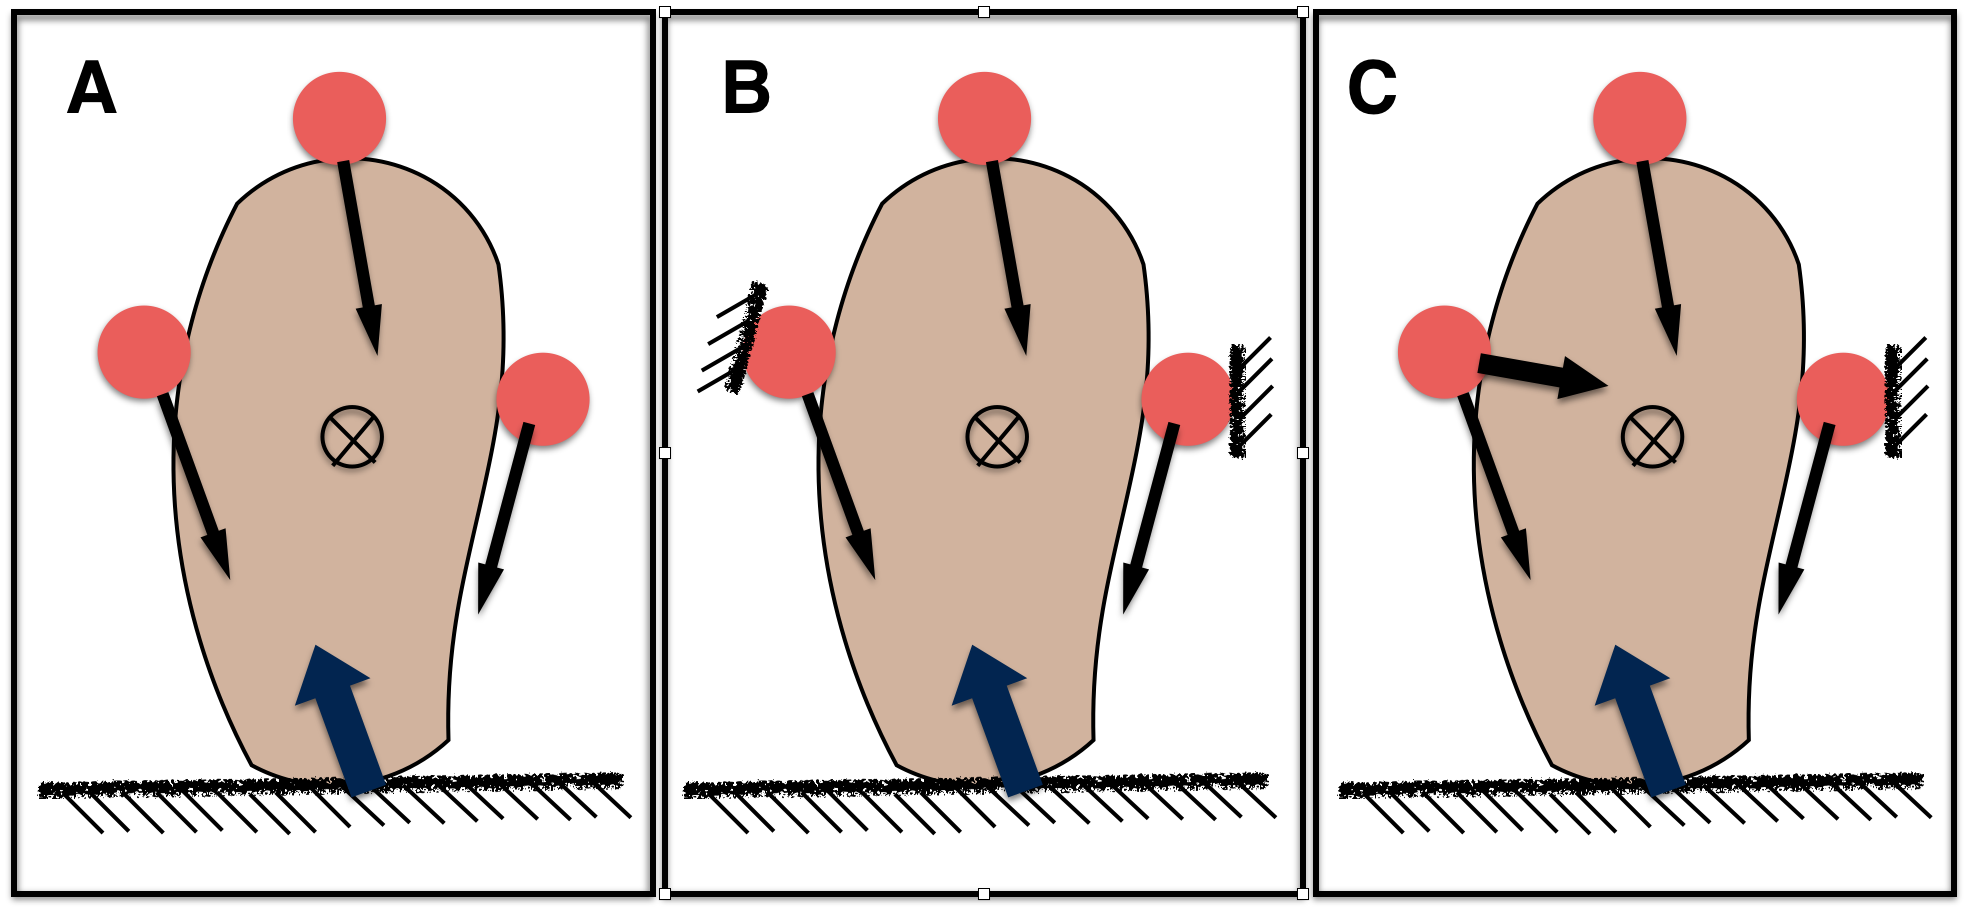
\includegraphics[width=4in]{./figs/pushExample.png}}
\end{center}
\caption[]{Several designs with the goal of robust pushing.}
\label{PushExample}
\end{figure}

\begin{figure}
\begin{center}
\begin{tabular}{l|c|c|c|c|c|c|c|}
Design & x0 & y0 & kx & ky & cost &	actuated x range &	actuated y range \\ \hline
(A) 4 tendons, no compliance&	-&	-&	-&	-&	1600	&(-4, 0)	&(-4, 0)\\
(B) 4 tendons, compliance	&-1.887	&-2.58	&0.54&	0.43&	{\bf 107.65} &	(-1.36, 1.02)	&(-1.61, 1.11) \\
(C) 2 tendons, spring open&	7	&7	&min	&min	&1600	&(-4, 0)	&(-4, 0)\\
(D) 2 tendons, spring closed&	-5.883&	-4.998&	0.45&	0.5	& {\bf 445.3}  &	(0, 2.65)&	(0, 2.49)
\end{tabular}
\end{center}
\caption{Optimal parameters, cost, and actuator range for several mechanism designs to perform Grasp A, Grasp B, and Manipulation 1.}
\label{ComplianceAnalysis}
\end{figure}

One keystone of our approach is strategic consideration of joint limits and compliance.  We illustrate the importance of these elements for the simple example.  Specifically, we show that (1) Careful design of compliance can reduce the number of actuators and actuator load, and (2) Joint limits can be important for robust performance.   Following this discussion, we present an approach to analyze grasps and manipulations to properly consider joint limits (Section \ref{secLimitAnalysis}) and approaches for design optimization to handle much more complex Grasp Nets to accomplish tasks such as those shown in Figure \ref{DexterousExamples} (Section \ref{secHandDesign}).

\smallskip\noindent
{\bf (1) Compliance matters.}  Table~\ref{ComplianceAnalysis} shows parameters for four tendon driven designs, which were optimized to perform Grasp A, Grasp B, and Manipulation 1 for objects  having widths from 1 to 4 finger radii.   Quasistatic analysis was performed for each design, with actuators for the thumb moving in the X direction, and actuators for the finger moving in the Y direction.  The quasistatic analysis ensured that forces required for Grasp A, Grasp B, and Manipulation 1 could be generated by the mechanism.   Each design was optimized using CMA \cite{hansen2006cma} to require the minimum total actuation force, expressed as squared actuated forces summed over actuators, objects, and time samples.    Where compliance was considered, linear springs were assumed, with zero point and stiffness given as parameters to the optimizer.   Optimal parameters, cost, and range of actuated forces are shown in the Figure.

Design (A) contains 4 tendons, which give active control in the negative and positive X directions for the thumb and the negative and positive Y directions for the finger.   This design considers no passive compliance.   Design (B) contains the same 4 tendons, but it also includes linear springs.   Note that the cost of forces provided by the actuators is less than 7 percent that of Design (A).    Design (C) has two tendons which act to close the hand, with elastic return springs to open the hand.    The presence of the spring elements reduces the total number of actuators, but does not reduce the cost of the design.    Design (D) also has two tendons, which act to open the fingers.    In Design (D), the spring elements close the hand and provide grip force.  The cost of Design (D) is 28 percent of that of Design (A), and the design achieves this result with half the number of actuators.    Clearly, compliance matters.   If we are able to maintain 4 actuators, compliance allows us to reduce forces to a small fraction of their magnitude without compliance, even while handling a variety of object sizes.   Adding compliant elements makes it possible to reduce the number of actuators to two and {\it also} reduce forces to a fraction of their original value.  Fortunately, it has become increasingly easy to incorporate compliant elements into a design using 3D printing and other technologies, such that we can consider this just one more design element available to optimize.

\begin{figure}
\begin{center}
\begin{tabular}{l|c|c|c|c|c|}
Test Case & \multicolumn{5}{c}{Errors at Gaussian perturbation (radians)}  \\
                & None & 0.1  & 0.2  & 0.3  &  0.4  \\ \hline 
(A) Joint limits, learn with perfect mechanism &	{\bf 0.01} & 0.90 & 1.63 &	2.32 & 3.61 \\
(B) Joint limits, learn with perturbation	&  {\bf 0.04}	& {\bf 0.05}	& {\bf 0.08} &	{\bf 0.21} &	1.42 \\
(C) No joint limits, learn with perfect mechanism &	{\bf 0.01}	&	1.05&	2.13	& 2.84  &	4.06 \\
(D) No joint limits, learn with perturbation &	{\bf 0.03}	& {\bf 0.06} 	&1.43	&4.38	&5.75 \\
\end{tabular}
\end{center}
\caption{This exploration shows the value of joint limits.   Mean error of an optimized manipulation is shown as perturbations to the perfect mechanism grow in magnitude.    Standard deviation is in parentheses.  The test having both joint limits and optimized while seeing small perturbations is able to handle perturbations three time the size of any other situation tested.}
\label{JointLimitAnalysis}
\end{figure}

\smallskip\noindent
{\bf (2) Joint Limits matter.}   We observe that joint limits are not avoided in human motion.   In contrast, in the human system, joint limits and singularities are exploited.    The limit at our knee that facilitates straight leg walking is a well known example, but there are many examples in grasping and manipulation as well.  In a lateral grasp (which motivated Grasp B), the moderately flexed fingers can passively support large forces, even though the force that can be actively generated by the fingers in that grasp is small, coming from small intrinsic muscles in the hand, such as the interossei \cite{brand1999clinical}.   The large grasp forces are available because the fingers are operating near their joint limits in this direction.   As another example, large forces can be transmitted through our palm all the way up to our strong shoulder muscles, or even through to the ground in some cases.   Pressing hard with a fingertip also exploits joint limits.

Here, we show one simple example that joint limits can make a practical difference.   In this set of tests, we explored the ability to learn robust open loop control for Manipulation 1.    Motor velocities for the thumb and finger were represented as linear functions of time, with three velocity control points per finger, resulting in a search space of six parameters.   CMA was used to optimize these parameters.    Box2D \cite{catto2011box2d} was used to simulate the manipulation for any given parameter set.   The cost at the end of each simulation was the difference between the final object configuration and that desired for Grasp B.     Once an optimal open loop motion had been identified by the optimizer, it was evaluated on a series of 5 test sets, each involving 100 simulations having perturbations in the direction of motion of the finger.    Finger motion direction was perturbed about its intended direction using a normal distribution with standard deviation of 0, 0.1, 0.2, 0.3, and 0.4 radians.    The motivation for this choice is that in a more complex hand, it is often difficult to know exactly where the fingers are relative to one another, and this variation can affect ability to manipulate robustly.   When a test used joint limits, the limits for the thumb were placed in the X direction, both at the thumb's origin in Grasp A and at a wide open position that gave clearance twice the width of the largest object.   Joint limits for the finger, when used, were placed in the Y direction, both at its destination in Grasp B and in a wide open position that gave clearance twice the width of the largest object.

Four cases were considered (Figure~\ref{JointLimitAnalysis}).   In Case (A), joint limits were included, and the manipulation action was optimized assuming a perfect mechanism.   Case (B) is similar to Case (A), but included random perturbations during the learning phase, having a standard deviation of 0.2 radians.    In cases (C) and (D), joint limits are not included.   Figure~\ref{JointLimitAnalysis} shows the results.   Empirically, results with error less than 0.5 in our scale produced consistently good manipulations.   These results show that when a task is optimized assuming a perfect mechanism, the effect of joint limits is not clear.    However, when the optimization process has the opportunity to see perturbations, the optimizer learns to use the joint limits to create robust strategies.    Case (B), including both joint limits and learning with perturbations, is able to handle three times the amount of disturbance of any other case.      Here, clearly joint limits matter.  Intuitively, this is because driving a joint to its limit reduces uncertainty and reduces the need for control to be exact (i.e., many controls can drive the joint to its limit).   Whenever such limits can be used, they offer great advantage.   Fortunately, it is easy to build in joint limits as well, as part of shape optimization.   For our instantiation of the Simple Example, we used geometric features to limit range of motion of the fingers.

In addition to joint limits and compliance, there are of course other things that matter.   One design element is shape.   Consider, for example, how we can make good use of our palm and its ability to conform.    Another is surface properties.   It may be beneficial to have some parts of the hand be slippery and others have high friction.   For example, in the Simple Example we had the object slide on the finger and roll on the thumb.   Another aspect is ability to sense unexpected slip, force, or motion.    We propose to investigate these options in the context of the larger goal of dexterous manipulation.


\section{Grasp and Manipulation Analysis with Joint Limits}
   \label{secLimitAnalysis}

One research challenge addressed in this proposal is to expand our analysis tools to deal well with joint limits.   We illustrate the problem and sketch a solution through the simple example in Figure~\ref{PushExample}.   Consider first Figure~\ref{PushExample} A.     The goal is to push into a surface, holding the object in the given grasp.   There will be variation in the task, as the object may contact the surface at different points and with different surface contact normals, resulting in varying force directions and moment about the object center of mass.   The Figure shows just a single example of task forces that could be encountered.    Each finger has one tendon to actuate it, with directions of actuation shown.    We assume the two fingers on the sides have considerable compliance in the horizontal direction.   Actuating these fingers does not help, as this will only cause the fingers to slide along the object surface.    With the design as shown in Figure~\ref{PushExample} A, the grasp will only be able to apply a very small range of task related forces to the object.

We can examine the force balance equations.   Because the fingers are very compliant, forces on the fingers must be balanced to prevent them from moving:
\begin{equation}
    f_{s, i} +     f_{a, i} +     f_{JL, i} +     f_{c, i} = 0
\end{equation}
Parameter $f_{s, i}$ is the spring force, with a component due to deviation of the initial contact location $c_i$ from rest position $c_{i, 0}$ and a second component due to object motion that results from unequalized forces $\Delta X_o$, which is intended to be small for a good grasp.   Matrix $K_i$ encodes stiffness as seen at the fingertip and $G_i$ is the grasp matrix for finger i.
\begin{equation}
 f_{s, i} = -K_i ( c_i - c_{i, 0}) - K_i G^T_i \Delta X_o
\end{equation}
Parameter $f_{a, i} = D_i P_i A_i$ is force generated by the actuators as in \cite{Li:graspDB07}, and is expressed using activation levels $A_i$, $0 \leq a_i \leq 1$, diagonal matrix $P_i$ of maximum actuator forces, and matrix $D_i$ of actuator directions.

\smallskip
\noindent
Parameter $f_{JL, i}$ is the novel component compared to other treatments that consider grasp quality for compliant systems (e.g., \cite{lin2000stiffness}), and can be expressed for a frictionless joint limit surface as:
\begin{equation}
	f_{JL, i} = -k_{JL} N_i S_i N^T_i      G^T_i \Delta X_o
\end{equation}
with joint limit normal matrix $N_i$ and (large) stiffness experienced at the limit of $k_{JL}$.    Note the selector matrix $S_i$ which indicates which joint limits relevant to finger i are currently engaged by some external or active force.

\smallskip
\noindent
Parameter $f_{c, i}$ is the contact force, which must be within the friction cone at the contact and contributes to balancing a desired external wrench $W_{ext}$ due to the pushing contact with the ground in this case:
\begin{equation}
  - \sum_i G_i f_{c, i} = W_{ext}
\end{equation}
For a given value of selector matrices $S_i$, we can solve the resulting linear system for actuator forces $A$ and object motion $\Delta X_o$.    In a valid solution, $\Delta X_o$ must be consistent with selection matrix $S_i$ such that the object motion pushes the object into the limit to engage it.   The system as a whole can be resolved through pivoting or other discrete search techniques.

A similar analysis gives guidance for design of joint limits.  Following \cite{Li:graspDB07} we can identify the worst case task wrench.   Knowing this wrench, we can attempt to place a joint limit to oppose it.   To visualize this process, note that in two dimensions a task wrench is a line with direction and moment about the origin.  We wish to identify the joint limit to supply the opposing wrench nearest to this line, with the added consideration that task wrenches or other actuators must engage this limit.
 
In the case shown in Figure~\ref{PushExample}, a search for optimal joint limits may result in Figure~\ref{PushExample} B, which is similar to using two fingers laterally as guides while pushing with a middle finger.   Here, the range of task forces that can be applied is considerably greater.     Torques due to ground contact forces at the object base engage one of the joint limits, allowing a force balance to be created.

A third option, shown in Figure~\ref{PushExample} C, is to add an additional actuator that can actively engage the joint limit opposite to it.   The result is a very strong grasp, reminiscent of human power lateral grasps, which can easily provide the task forces and many more.   As a side benefit, the two previously useless actuators can now contribute to the task, sharing the load with the actuator of the top finger.

In each case, the force balance equation as shown here, along with a straightforward linear optimization, have made it possible to evaluate the effect of any new design element on the ability of the push grasp to achieve task forces.

Extension to complex and redundant mechanisms is more complex but can follow the same line of reasoning.   Developing and evaluating these analysis tools is one task of the proposed research.
